\chapter{Experiments}\label{ch:experiments}
%look at experiment introduction in Grzes phd thesis

In this chapter we give experimental evidence of the goodness of our approach, discussed mainly in Chapter \ref{ch:rl} and \ref{ch:reward-shaping}, by using the implementations presented in Chapter \ref{ch:flloat} and \ref{ch:rltg}. For each considered environment, we give a formal description in the framework of MDPs and assign temporal goals to be satisfied, as explained in earlier chapters.
\section{\Breakout}
In this section, we use the \Breakout environment (already presented in Example \ref{exa:breakout}). We first show how the combination of temporal goals is successfully learnt by the agent. Then, we show a benchmarking between the use of off-line reward shaping, on-the-fly reward shaping and no reward shaping.
\paragraph{Description of the Environment:}
The actions available to the agent are \emph{left}, \emph{right} and \emph{no-action}. The relevant features are: position of the paddle $p_x$, position of the ball $b_x, b_y$, speed of the ball $v_x, v_y$ and status of each brick (booleans) $b_{ij}$. These features of the system give all the needed informations to predict the next state from the current state. Hence we can build an MDP where: $\States$ is the set of  all the possible values of the sequence of features $\tup{p_x, b_x, b_y, v_x, v_y}$, $\Actions = \set{\text{\emph{right, left, no-action}}}$, transition function $\TrFun$ determined by the rules of the game. We give reward $R(s,a,s')=10$ if a particular brick in $s'$ has been removed for the first time, plus $100$ if that brick was the last (i.e. \emph{environment goal} reached).

\paragraph{Temporal goal:} The \emph{temporal goal} (specified by a \LLf formula) is to remove lines of bricks in a given order. In other words, all bricks on each line of bricks $i$ must be removed before removing all bricks from line $j > i$.
In our experiments we considered the following goals (and combinations of them):

\begin{itemize}
	\item \textsc{Break-Cols-(LR|RL)}:  remove columns of blocks from (left to right | right to left).
	\item \textsc{Break-Rows-(BT|TB)}:  remove rows of blocks from (bottom to top | top to bottom).
\end{itemize}

For each temporal goal, we give a reward $r = 10000$ and it is given when the agent fulfilled the temporal goal specified by the formula.
The formulas are expressed in \LDLf. For example, in Breakout 3x3 (i.e. three rows and three columns of bricks), the formula which specify the just explained temporal goals is:
\begin{equation}\label{eq:breakout-temporal-goal}
\DIAM{(\lnot l_0 \lAND \lnot l_1 \lAND \lnot l_2)^*;(l_0 \lAND \lnot l_1 \lAND \lnot l_2);(l_0 \lAND \lnot l_1 \lAND \lnot l_2)^*;(l_0 \lAND l_1 \lAND \lnot l_2);(l_0 \lAND l_1 \lAND \lnot l_2)^*;(l_0 \lAND l_1 \lAND l_2)}tt
\end{equation}
where the fluent $l_i$ means "the $i_{th}$ line has been removed".
The automaton associated to the formula in Equation \ref{eq:breakout-temporal-goal} is depicted in Figure \ref{fig:breakout-automaton}. $l_i$ are the fluents of interests, hence $\Prop = \set{l_0, l_1, l_2}$ and $\L = 2^\Prop$.

\begin{figure}[h]
	\centering
	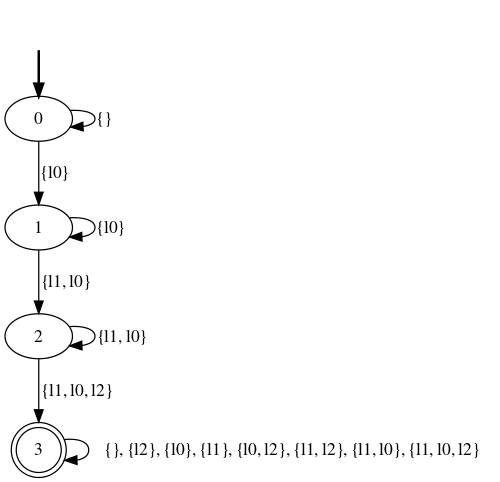
\includegraphics[width=0.6\textwidth]{images/breakout.png}
 	\caption{The automaton associated to the \LDLf formula in Equation \ref{eq:breakout-temporal-goal} for \Breakout 3x3.}
 	\label{fig:breakout-automaton}
\end{figure}

The features for fluents evaluation, for every temporal goal, are the status of each brick (present or removed). Recalling the notation used in Example \ref{exa:breakout}: $\tup{b_{11}, \dots, b_{nm}}$.

It is crucial to remark that the evaluation of the fluent from the features is different among the temporal goals above mentioned, despite the formulas are structurally the same (apart from the number of lines to remove). Indeed, thanks to the fluents evaluation phase (i.e. the map from features values to the truth of each fluent), the formulas behave differently.

\paragraph{Configurations:}
The reinforcement algorithm used is Sarsa$(\lambda)$ (e.g. Sarsa with eligibility traces) with $\epsilon$-greedy policy. The values of the parameters are:
\begin{itemize}
	 \item $\lambda = 0.99$
	 \item $\DiscFact=0.999$	
	 \item $\alpha=0.1$
	 \item $\epsilon= 0.1$
\end{itemize}

The experiments are stopped when in the last 100 episodes of optimal runs the agent always achieved both the environment goal and the temporal goals.
Notice that this approach may yield a sub-optimal policy, but the found policies always satisfy \LLf goals. This method is used also for the other experiments.

\subsection{Optimal policies}
Now we show some screenshots of the optimal policies found for some of the temporal goals described before. You can find full recordings at \url{https://www.youtube.com/channel/UChpe0QEtRSKh4uCy5f2XuGA}.

\subsubsection{\textsc{Break-Cols-LR}}
In Figure \ref{exa:breakout-33-lr} are depicted the highlights of a run of the optimal policy for the goal \textsc{Break-Cols-LR}. As you can notice, the constraint expressed by the formula in Equation \ref{eq:breakout-temporal-goal} is satisfied (i.e. the columns of bricks are broken from left to right).

\begin{figure}[h]
	\centering
	\begin{subfigure}[b]{0.23\textwidth}
		
\includegraphics[width=\textwidth]{images/breakout-33-lr-1.png}
		%	 	\caption{a}
		%	 	\label{a}
	\end{subfigure}
	~ %add desired spacing between images, e. g. ~, \quad, \qquad, \hfill etc. 
	%(or a blank line to force the subfigure onto a new line)
	\begin{subfigure}[b]{0.23\textwidth}
		
\includegraphics[width=\textwidth]{images/breakout-33-lr-2bis.png}
		%	 	\caption{}
		%	 	\label{}
	\end{subfigure}
	~ %add desired spacing between images, e. g. ~, \quad, \qquad, \hfill etc. 
	%(or a blank line to force the subfigure onto a new line)
	\begin{subfigure}[b]{0.23\textwidth}
		
\includegraphics[width=\textwidth]{images/breakout-33-lr-2.png}
		%	 	\caption{}
		%	 	\label{}
	\end{subfigure}
	\begin{subfigure}[b]{0.23\textwidth}
		
\includegraphics[width=\textwidth]{images/breakout-33-lr-3.png}
		%	 	\caption{}
		%	 	\label{}
	\end{subfigure}
	\caption{A run of the learnt optimal policy for the task \textsc{Break-Cols-LR}. From left to right, you can see that the columns are broken in the right order.}\label{exa:breakout-33-lr}
\end{figure}

\subsubsection{\textsc{Break-Cols-BT}}
In Figure \ref{exa:breakout-33-bt} are depicted the highlights of a run of the optimal policy for the goal \textsc{Break-Cols-BT}. The constraint expressed by the formula in Equation \ref{eq:breakout-temporal-goal} is satisfied (i.e. the rows of bricks are broken from the bottom to the top).


\begin{figure}[h]
	\centering
	\begin{subfigure}[b]{0.23\textwidth}
		
\includegraphics[width=\textwidth]{images/breakout-33-bt-1.png}
		%	 	\caption{a}
		%	 	\label{a}
	\end{subfigure}
	~ %add desired spacing between images, e. g. ~, \quad, \qquad, \hfill etc. 
	%(or a blank line to force the subfigure onto a new line)
	\begin{subfigure}[b]{0.23\textwidth}
		
\includegraphics[width=\textwidth]{images/breakout-33-bt-2bis.png}
		%	 	\caption{}
		%	 	\label{}
	\end{subfigure}
	~ %add desired spacing between images, e. g. ~, \quad, \qquad, \hfill etc. 
	%(or a blank line to force the subfigure onto a new line)
	\begin{subfigure}[b]{0.23\textwidth}
		
\includegraphics[width=\textwidth]{images/breakout-33-bt-2.png}
		%	 	\caption{}
		%	 	\label{}
	\end{subfigure}
	\begin{subfigure}[b]{0.23\textwidth}
		
\includegraphics[width=\textwidth]{images/breakout-33-bt-3.png}
		%	 	\caption{}
		%	 	\label{}
	\end{subfigure}
	\caption{A run of the learnt optimal policy for the task \textsc{Break-Rows-BT}. From the bottom to the top, you can see that the rows are broken in the right order.}\label{exa:breakout-33-bt}
\end{figure}


\subsubsection{\textsc{Break-Cols-RL-TB}}
In Figure \ref{exa:breakout-33-rl-tb} are depicted the highlights of a run of the optimal policy for the goal \textsc{Break-Cols-RL-TB}. Notice that, even in the case of multiple temporal goals, the constraints expressed by the formula in Equation \ref{eq:breakout-temporal-goal} are satisfied (i.e. the rows of bricks are broken from the top to the bottom and the columns of bricks are broken from right to left). Furthermore, notice that the formula is the same, but \emph{how the fluents are evaluated from the features}  makes the difference.


\begin{figure}[h]
	\centering
	\begin{subfigure}[b]{0.18\textwidth}
		
\includegraphics[width=\textwidth]{images/breakout-33-rl-tb-1.png}
		%	 	\caption{a}
		%	 	\label{a}
	\end{subfigure}
	~ %add desired spacing between images, e. g. ~, \quad, \qquad, \hfill etc. 
	%(or a blank line to force the subfigure onto a new line)
	\begin{subfigure}[b]{0.18\textwidth}
		
\includegraphics[width=\textwidth]{images/breakout-33-rl-tb-2.png}
		%	 	\caption{}
		%	 	\label{}
	\end{subfigure}
	~ %add desired spacing between images, e. g. ~, \quad, \qquad, \hfill etc. 
	%(or a blank line to force the subfigure onto a new line)
	\begin{subfigure}[b]{0.18\textwidth}
		
\includegraphics[width=\textwidth]{images/breakout-33-rl-tb-3.png}
		%	 	\caption{}
		%	 	\label{}
	\end{subfigure}
	\begin{subfigure}[b]{0.18\textwidth}
		
\includegraphics[width=\textwidth]{images/breakout-33-rl-tb-4.png}
		%	 	\caption{}
		%	 	\label{}
	\end{subfigure}
	\begin{subfigure}[b]{0.18\textwidth}
		
\includegraphics[width=\textwidth]{images/breakout-33-rl-tb-5.png}
		%	 	\caption{}
		%	 	\label{}
	\end{subfigure}
	\caption{A run of the learnt optimal policy for the task \textsc{Break-Cols-RL-TB}. You can see that the rows are broken from the top to the bottom and that, at the same time, the columns are broken from the right to the left.}\label{exa:breakout-33-rl-tb}
\end{figure}

\subsection{Benchmarking of reward shaping techniques}\label{sect:breakout-benchmarking-rs}
In this section, we report some statistics about the performances of the proposed approach with a focus on automata-based reward shaping.
For each configuration, we collected the observed reward for each episode, over 10 runs. Each run has a time limit of 10000 episodes.
Then we moving averaged the sequences of rewards with a window of size 100, in order to make the curves more smoothed, and averaged the result across all the runs. The plots show this processed sequences over the number of episodes. The coloured bands represent the 90\% confidence interval taken from bootstrapped re-samples.

We show our results in two parts:
\begin{enumerate}
	\item Comparison of \emph{No Reward Shaping}, \emph{Off-line Reward Shaping} and \emph{On-the-fly Reward Shaping} in \Breakout 3x3, 3x4 and 4x4, with temporal goal \textsc{Break-Cols-LR};
	\item Comparison of \emph{No Reward Shaping}, \emph{Off-line Reward Shaping} and \emph{On-the-fly Reward Shaping} in Breakout 4x4, with temporal goals \textsc{Break-Cols-LR}, \textsc{Break-Rows-BT}, \textsc{Break-Cols-LR \& Break-Rows-BT};
\end{enumerate}

\subsubsection{Different number of bricks and rows}
In Figure \ref{fig:breakout-benchmarking-reward-shaping-lr-different-bricks} are plotted different statistics by increasing difficulty in the environment, for every variant of reward shaping technique.
On the x-axis the number of episodes, on the y-axis the average reward (obtained as explained above). In every case, we can see that the use of reward shaping (both off-line and on-the-fly) speed-up the learning process.
\begin{figure}[h]
	 \centering
	 \begin{subfigure}[b]{0.65\textwidth}
	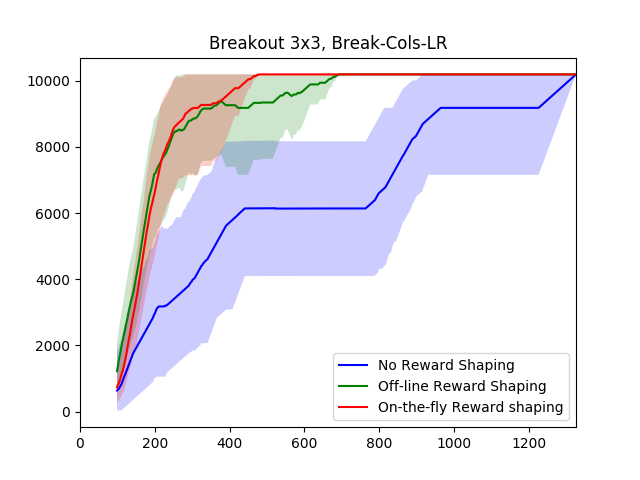
\includegraphics[width=\textwidth]{images/rs-comparison_b33.png}
	 	\caption{\Breakout 3x3, \textsc{Break-Cols-LR} for three different settings: \emph{No RS}, \emph{Off-line RS} and \emph{On-the-fly RS}}
	 	\label{fig:breakout-benchmarking-reward-shaping-33-lr}
	 \end{subfigure}
	 ~ %add desired spacing between images, e. g. ~, \quad, \qquad, \hfill etc. 
	 %(or a blank line to force the subfigure onto a new line)
	 \begin{subfigure}[b]{0.65\textwidth}
		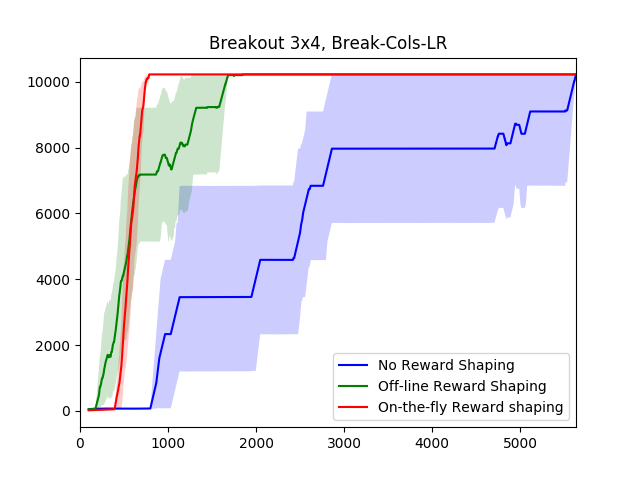
\includegraphics[width=\textwidth]{images/rs-comparison_b34.png}
	 	\caption{\Breakout 3x4, \textsc{Break-Cols-LR} for three different settings: \emph{No RS}, \emph{Off-line RS} and \emph{On-the-fly RS}}
	 	\label{fig:breakout-benchmarking-reward-shaping-34-lr}
	 \end{subfigure}
	 ~ %add desired spacing between images, e. g. ~, \quad, \qquad, \hfill etc. 
	 %(or a blank line to force the subfigure onto a new line)
	 \begin{subfigure}[b]{0.65\textwidth}
	 	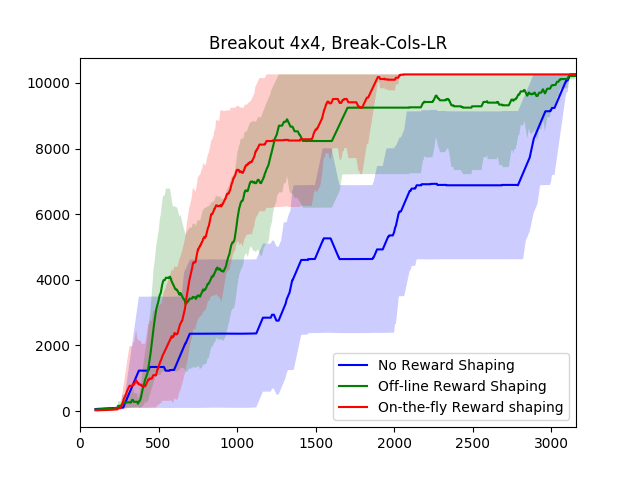
\includegraphics[width=\textwidth]{images/rs-comparison_b44.png}
	 	\caption{\Breakout 4x4, \textsc{Break-Cols-LR} for three different settings: \emph{No RS}, \emph{Off-line RS} and \emph{On-the-fly RS}}
	 	\label{fig:breakout-benchmarking-reward-shaping-44-lr}
	 \end{subfigure}
	 \caption{The results of three settings are reported, namely: \Breakout 3x3, 3x4 and 4x4 (\ref{fig:breakout-benchmarking-reward-shaping-33-lr}, \ref{fig:breakout-benchmarking-reward-shaping-34-lr} and  \ref{fig:breakout-benchmarking-reward-shaping-44-lr} respectively), all of them with temporal goal \textsc{Break-Cols-LR}. On the x-axis the episodes, on the y-axis the average reward.In every case, we can see that the use of reward shaping (both off-line and on-the-fly) speed-up the learning process. }\label{fig:breakout-benchmarking-reward-shaping-lr-different-bricks}
\end{figure}


\subsubsection{Different temporal goals}
In Figure \ref{fig:breakout-benchmarking-reward-shaping-44-different-goal} Here we show the performances by varying the temporal goals.
On the x-axis the number of episodes, on the y-axis the average reward (obtained as explained above). In every case, we can see that the use of reward shaping (both off-line and on-the-fly) speed-up the learning process.
\begin{figure}[h]
	\centering
	\begin{subfigure}[b]{0.65\textwidth}
		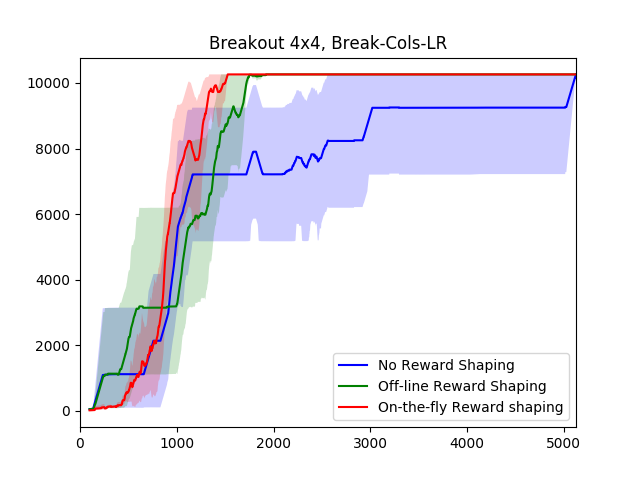
\includegraphics[width=\textwidth]{images/b44-cols-comparison}
	 	\caption{\Breakout 4x4, \textsc{Break-Cols-LR} for three different settings: \emph{No RS}, \emph{Off-line RS} and \emph{On-the-fly RS}}
		\label{fig:breakout-benchmarking-reward-shaping-44-lr-varying-goal}
	\end{subfigure}
	~ %add desired spacing between images, e. g. ~, \quad, \qquad, \hfill etc. 
	%(or a blank line to force the subfigure onto a new line)
	\begin{subfigure}[b]{0.65\textwidth}
		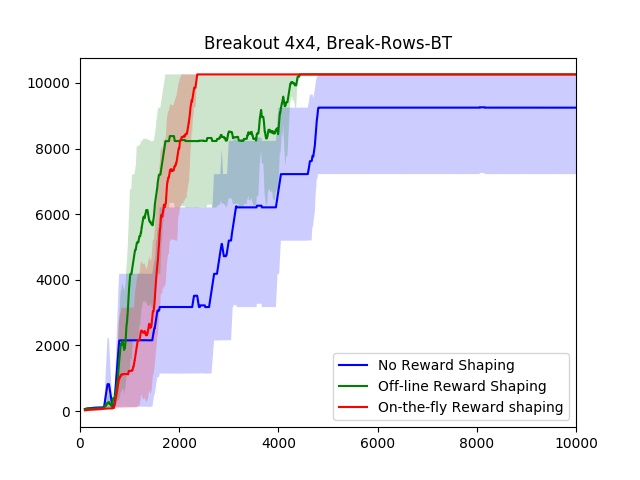
\includegraphics[width=\textwidth]{images/b44-rows-comparison}
	 	\caption{\Breakout 4x4, \textsc{Break-Rows-BT} for three different settings: \emph{No RS}, \emph{Off-line RS} and \emph{On-the-fly RS}}
		\label{fig:breakout-benchmarking-reward-shaping-44-bt-varying-goal}
	\end{subfigure}
	~ %add desired spacing between images, e. g. ~, \quad, \qquad, \hfill etc. 
	%(or a blank line to force the subfigure onto a new line)
	\begin{subfigure}[b]{0.65\textwidth}
		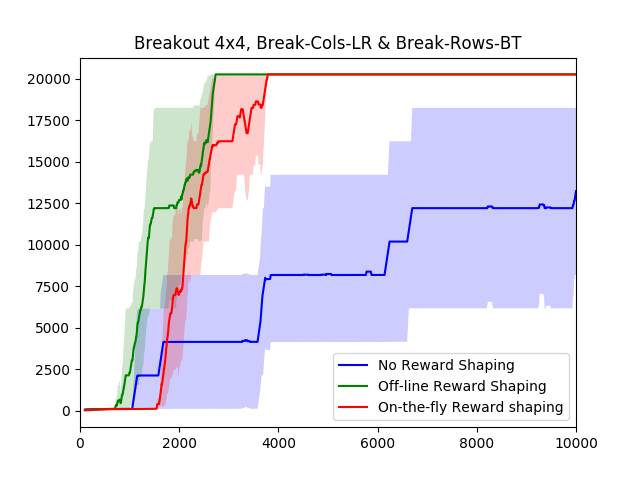
\includegraphics[width=\textwidth]{images/b44-both-comparison}
		\caption{\Breakout 4x4, \textsc{Break-Cols-LR \& Break-Rows-LR} for three different settings: \emph{No RS}, \emph{Off-line RS} and \emph{On-the-fly RS}}
		\label{fig:breakout-benchmarking-reward-shaping-44-lr-bt-varying-goal}
	\end{subfigure}
	\caption{The results of three settings are reported, namely: \Breakout 4x4 with temporal goal \textsc{Break-Cols-LR}, \textsc{Break-Cols-BT} and \textsc{Break-Cols-LR \& \textsc{Break-Cols-BT}} (\ref{fig:breakout-benchmarking-reward-shaping-44-lr-varying-goal}, \ref{fig:breakout-benchmarking-reward-shaping-44-bt-varying-goal} and  \ref{fig:breakout-benchmarking-reward-shaping-44-lr-bt-varying-goal} respectively). On the x-axis the episodes, on the y-axis the average reward. In every case, we can see that the use of reward shaping (both off-line and on-the-fly) speed-up the learning process. }\label{fig:breakout-benchmarking-reward-shaping-44-different-goal}
\end{figure}
\clearpage

\section{\Sapientino}
\Sapientino Doc is an educational
game for 5-8 y.o. children in which a small mobile robot
has to be programmed in order to visit specific cells in a 5x7
grid. Cells contain concepts that must be matched by the
children (e.g., a coloured animal, a colour, and the initial letter
of the name of the animal). The robot executes sequences of actions given in input by children with a keyboard on the
robot's top side. During execution, the robot moves on the
grid and executes an action (actually a \emph{bip}) to announce that
the current cell has been reached (this is called a \emph{visit} of a
cell). In this paper, we
generalize this game as follows. As in the real game, we consider a 5x7 grid with 7 triplets of coloured cells, each triplet
representing three matching concepts (see Figure \ref{fig:sapientino-screenshot} for a screenshot).

\begin{figure}[h]
	\centering
	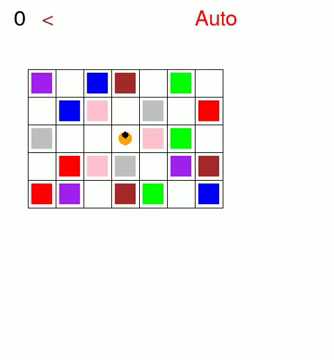
\includegraphics[width=0.5\textwidth]{images/sapientino-start-screen.png}
	\caption{A screenshot from \Sapientino}
	\label{fig:sapientino-screenshot}
\end{figure}

\paragraph{Actions, Features and Fluents:}  The actions available to the agent are: \textsc{up, down, left, right} and \textsc{bip}. The features for the agent space are the position $(x,y)$ of the agent in the grid, namely $f_x$ and $f_y$. The features for evaluating the fluents configurations are: $f_b$ reporting if a \textsc{bip} has just been executed, and $f_c$ denoting the colour of the current cell. In our setting, the available fluents are: $$\Prop = \set{bip, red, green, blue, pink, brown, grey, purple}$$ with the obvious meaning that their name indicates (just map features to fluents one-to-one).

\paragraph{Temporal Goal:} In our experiment, we considered the following temporal behaviours:
\begin{itemize}
	\item \textsc{Ordered-Visits}: \emph{visit} each colour and do a \emph{bip} in each colour in a given order.
	\item \textsc{Illegal-Bips}: between each visit, never do a \emph{bip}. 
\end{itemize}

We identified two temporal goals: one considering that both conditions must be satisfied and a more relaxed one that only \textsc{Ordered-Visits} must be satisfied. They can be translated, respectively, into the following \LDLf formulas:

\begin{align}\label{eq:sapientino-temporal-goal}
\DIAM{&(\lnot bip)^*;red \lAND bip;(\lnot bip)^*;green \lAND bip;& \nonumber\\
&(\lnot bip)^*;blue \lAND bip;(\lnot bip)^*;pink \lAND bip;& \nonumber\\
&(\lnot bip)^*;brown \lAND bip;(\lnot bip)^*;grey \lAND bip;&\nonumber\\
&(\lnot bip)^*;purple \lAND bip}tt
\end{align}

and: 
\begin{align}\label{eq:sapientino-temporal-goal-relaxed}
\DIAM{&\true^*;red \lAND bip;\true^*;green \lAND bip;& \nonumber\\
	&\true^*;blue \lAND bip;\true^*;pink \lAND bip;& \nonumber\\
	&\true^*;brown \lAND bip;\true^*;grey \lAND bip;&\nonumber\\
	&\true^*;purple \lAND bip}tt
\end{align}
where Formula \ref{eq:sapientino-temporal-goal-relaxed} is the same of Formula \ref{eq:sapientino-temporal-goal} but replacing every occurrence of  $(\lnot bip)^*$ with $\true^*$. The associated automaton are depicted, respectively, in Figure \ref{fig:sapientino-automaton} and \ref{fig:sapientino-relaxed-automaton}.
\begin{figure}[h]
	\begin{subfigure}{0.5\textwidth}
		\centering
		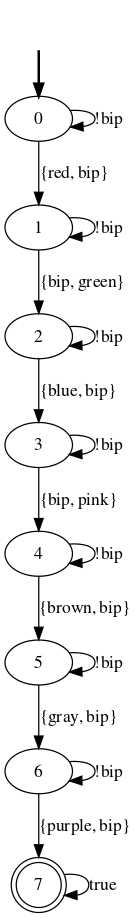
\includegraphics[width=0.21\textwidth]{images/sapientino_ldlf.png}
		\caption{The automaton associated to the \LDLf formula in Equation \ref{eq:sapientino-temporal-goal} for for the "full" temporal goal in \Sapientino.}
		\label{fig:sapientino-automaton}
	\end{subfigure}
	\begin{subfigure}{0.5\textwidth}
		\centering
		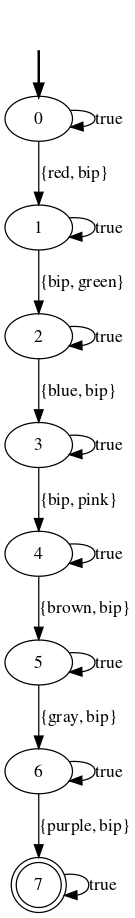
\includegraphics[width=0.21\textwidth]{images/sapientino_ldlf_relaxed.png}
		\caption{The automaton associated to the \LDLf formula in Equation \ref{eq:sapientino-temporal-goal-relaxed} for the "relaxed" temporal goal in \Sapientino.}
		\label{fig:sapientino-relaxed-automaton}
	\end{subfigure}

\end{figure}

Notice that the condition of illegal bips does not affect the optimal policy; on the other hand, it highly affects the exploration phase, since with the \textsc{Illegal-Bips} condition, every time the $\epsilon$-greedy policy chooses $bip$ randomly and "illegally", then that trajectory cannot satisfy the temporal goal anymore.  Moreover, observe that, in this case, we do not consider any \emph{environment goal}, as we did in \Breakout experiments (i.e. break all the bricks).
\paragraph{Configurations:}
The reinforcement algorithm used is Sarsa$(\lambda)$ (e.g. Sarsa with eligibility traces) with $\epsilon$-greedy policy. The values of the parameters are:
\begin{itemize}
	\item $\lambda = 0$
	\item $\DiscFact=1.0$	
	\item $\alpha=0.1$
	\item $\epsilon= 0.1$
\end{itemize}

\medskip


We show our results in two parts:
\begin{enumerate}
	\item Comparison of \emph{No Reward Shaping}, \emph{Off-line Reward Shaping} and \emph{On-the-fly Reward Shaping} in \Sapientino with the "full" temporal goal, i.e. \textsc{Ordered-Visits \& Illegal-Bips}\label{sapientino-experiment-configuration-1};
	\item Comparison of \emph{No Reward Shaping}, \emph{Off-line Reward Shaping} and \emph{On-the-fly Reward Shaping} in \Sapientino with the "relaxed" temporal goal, i.e. only \textsc{Ordered-Visits} \label{sapientino-experiment-configuration-2};
\end{enumerate}


We analyze the results of Experiment \ref{sapientino-experiment-configuration-1} and \ref{sapientino-experiment-configuration-2}. As stated before, since the two experiments differ only for the exploration phase, the optimal policy that satisfies the goal is qualitatively the same. You might see the resulting learnt policy at \url{https://www.youtube.com/watch?v=ghBImtYMpVk}.

\subsection{\textsc{Ordered-Visits \& Illegal-Bips}}
In this experiment, we observed that the agent successfully learned the temporal goal, both in off-line and in on-the-fly reward shaping. The performances are pretty the same. Notice that, without reward shaping, in our simulations (5000 episodes), \emph{the agent never reached the goal}.
This is due mainly to the long sequence of actions that the agent has to take in order to accomplish the entire goal, considering that an illegal $bip$ lead to a failure of the goal and so the end of the episode. On the other hand, in the case of reward shaping, an illegal bip is punished because the episode ends and the agent collects the negative potential fall. Hence, the agent recognizes, earlier than no reward shaping configuration, that the illegal bip is a bad action.
\subsection{\textsc{Ordered-Visits}}
Also in this case, the agent learned the temporal goal, even in the case where no reward shaping was applied. It is interesting to note that a small change in the formula can affect drastically the learning process, due to exploration phase constraints.

\section{\Minecraft}
\Minecraft \citep{pmlr-v70-andreas17a} is a sort of 2D porting of the well-known 3D videogame \href{https://minecraft.net/en-us/}{Minecraft}. 
The agent can $get$ resources (e.g. $wood$, $grass$) and $use$ tools (e.g. $toolshed$, $workbench$) located on a grid (similarly to the grid in \Sapientino), and has to accomplish composite tasks. For instance, the task \emph{make a bed} is divided into the following sequence of subtasks: $get\_wood$, $use\_toolshed$, $get\_grass$, $used\_workbench$. In Figure \ref{fig:minecraft-screenshot} you can see a screenshot of the game.

\paragraph{Actions, Features and Fluents:}  The actions available to the agent are: \textsc{up, down, left, right}, \textsc{get} and \textsc{use}. The features for the agent space are the position $(x,y)$ of the agent in the grid, namely $f_x$ and $f_y$. The features for evaluate the fluents configurations are: $f_g$ reporting if a \textsc{get} has just been executed,  $f_u$ reporting if a \textsc{use} has just been executed, $f_\ell$ denoting the resource/tool available in the current location, and $f'_\ell$, if a resource has been taken and is available for the incoming tasks. In our setting, the available fluents are: $$\Prop = \set{get\_wood, get\_grass, get\_iron, use\_toolshed,use\_workbench, use\_factory}$$ 
when the agent is near a resource (i.e. $wood$, $grass$ or $iron$) and do a \textsc{get}, then the associated "get" fluent becomes true. Analogously for tools and the \textsc{use} action. When a task is completed and to do that some previously collected resource/tool has been used, then the resources are lost and has to be recollected again in order to accomplish other tasks.

\begin{figure}[h]
	\centering
	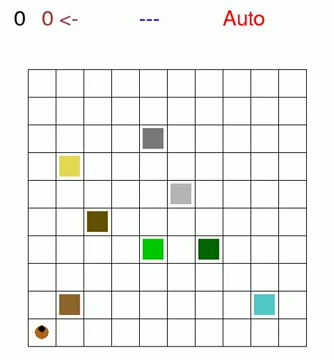
\includegraphics[width=0.5\textwidth]{images/minecraft-screenshot.png}
	\caption{A screenshot of the game \Minecraft}
	\label{fig:minecraft-screenshot}
\end{figure}

\paragraph{Temporal Goal:} In our experiment, we considered the following tasks:
\begin{enumerate}
	\item \textsc{Make-Bed}: $get\_wood, use\_toolshed, get\_grass, use\_workbench$\label{minecraft-goal-1}
	\item \textsc{Make-Axe}: $get\_wood, use\_workbench, get\_iron, use\_toolshed$\label{minecraft-goal-2}
	\item \textsc{Make-Bridge}: $get\_iron, get\_wood, use\_factory$\label{minecraft-goal-3}
\end{enumerate}
Now we show how to express them in \LDLf and its associated automaton. For simplicity, we show only the ones for the goal \ref{minecraft-goal-3}.
The associated \LDLf formula is:
\begin{align}\label{minecraft-goal-3-formula}
\DIAM{true^*}
\DIAM{&true^*;get\_iron \lAND \lnot get\_wood \lAND \lnot use\_factory;\nonumber\\
	&
	(get\_iron \lAND \lnot get\_wood \lAND \lnot use\_factory)^*;
	get\_iron \lAND get\_wood \lAND \lnot use\_factory;\nonumber\\
	&(get\_iron \lAND  get\_wood \lAND\lnot use\_factory)^*;
	get\_iron \lAND  get\_wood \lAND  use\_factory}tt
\end{align}
whereas the translation of Formula \ref{minecraft-goal-3-formula} into automaton is depicted in Figure \ref{fig:minecraft-goal-3-automaton}:

\begin{figure}[h]
	\centering
	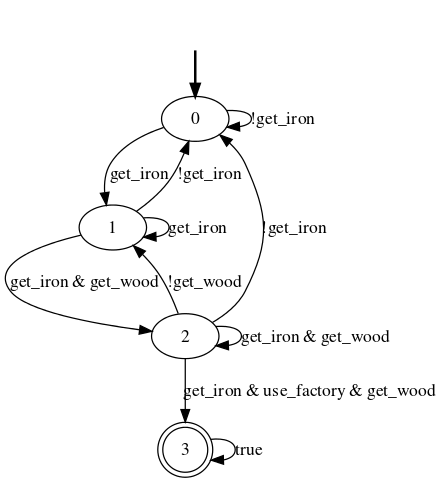
\includegraphics[width=0.5\textwidth]{images/minecraft_goal.png}
	\caption{An approximate representation of the automaton associated to Formula \ref{minecraft-goal-3-formula}. Notice that it is "simplified" by omitting groups of transitions that are collapsed in a single edge labeled with the propositional formula that the interpretation should satisfy.}
	\label{fig:minecraft-goal-3-automaton}
\end{figure}

Notice that we could "relax" the specified order of $get\_wood$ and $get\_iron$, since it is not relevant to the operation \emph{make a bridge}.

The agent is trained to satisfy all the three tasks in a single episode. For each temporal goal, the reward assigned is $1$.

\paragraph{Configurations:}
The reinforcement algorithm used is Sarsa$(\lambda)$ (e.g. Sarsa with eligibility traces) with $\epsilon$-greedy policy. The values of the parameters are:
	\begin{itemize}
		\item $\lambda = 0.9$
		\item $\DiscFact=0.99$	
		\item $\alpha=0.1$
		\item $\epsilon= 0.25$
	\end{itemize}

\subsection{Results}
In Figure \ref{fig:minecraft-comparison} is plotted the benchmarking, similarly to the one presented in Section \ref{sect:breakout-benchmarking-rs}. We notice that the policy that satisfies every temporal goal has been found when a reward shaping is applied, whereas in the case of no reward shaping the time limit imposed for the experiment was not enough to allow every run to achieve the goal. You can see one of these found policies at \url{https://youtu.be/IJ3Hr79xfBs}.

Observe that reward shaping, both in off-line and on-the-fly variant, outperform the absence of reward shaping. This is due mainly to the high number of steps that the agent has to make in a precise order in order to achieve the goal: without a guide in the exploration (e.g. shaping rewards) it is hard to discover the proper sequence that leads to the satisfaction of every formula. Furthermore, observe that off-line reward shaping is slightly better than on-the-fly reward shaping in terms of convergence rate. It is also more stable, as the reader might infer from the shaded regions that represent the variance of the plot: indeed, it is not surprising that on-the-fly reward shaping yields a more noisy learning process, due to the dynamic change of the potential function and so of the shaping rewards.

It is worth to notice the particular structure of the environment in our setting. Indeed, when one of the tasks is completed, the resources that progressed at the same time the other automata/tasks are released; this lead to a regression of the state of those tasks, and so to a negative shaping reward. Hence, the positive shaping reward given for progression is mitigated by the negative shaping reward due to completion of a task and regression of the other task that has some resource in common. The learning agent has to deal with this issue, that at the scaling of the problem it might lead to slow the learning.


\begin{figure}
	\centering
	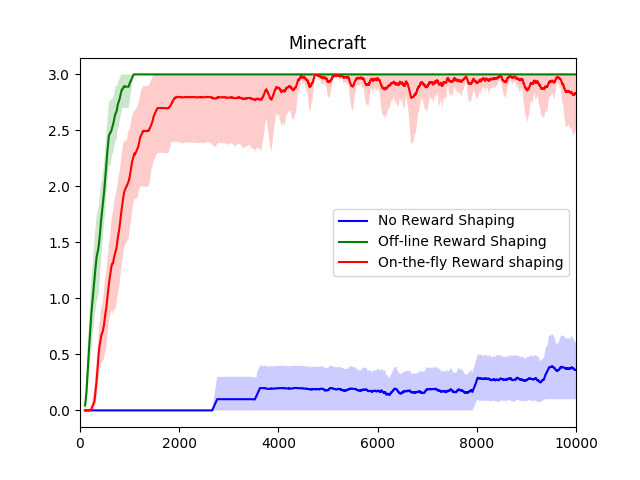
\includegraphics[width=0.8\textwidth]{images/minecraft-comparison.png}
	\caption{A comparison between reward shaping techniques for the temporal goals \ref{minecraft-goal-1}, \ref{minecraft-goal-2} and \ref{minecraft-goal-3}. On the x-axis the episodes, on the y-axis the average reward, as explained in Section \ref{sect:breakout-benchmarking-rs}.}
	\label{fig:minecraft-comparison}
\end{figure}


\section{Implementation}
The experiments are implemented using FLLOAT and RLTG, presented in Chapter \ref{ch:flloat} and Chapter \ref{ch:rltg}.
The code for running the experiments by yourself with other configurations and plot the statistics are published in \href{https://github.com/MarcoFavorito/rltg-examples}{this repository}. You'll find also the scripts to run the experiments analyzed in this chapter. The \Breakout, \Sapientino and \Minecraft implementations can be found in \href{https://github.com/MarcoFavorito/RLgames}{this repository}, which is a fork of \href{https://github.com/iocchi/RLgames}{this one}, created by \href{https://sites.google.com/a/dis.uniroma1.it/iocchi/home}{prof. Luca Iocchi}.